\documentclass[a4paper, 12pt]{article}

\usepackage[margin=2.5cm]{geometry}
\usepackage{indentfirst}
\usepackage{graphicx}
\usepackage{wrapfig}
\usepackage{amsmath}
\usepackage{mathrsfs}

\newcommand{\figcaption}[2]{\textbf{Fig. #1} #2}

\newcommand{\lorentzradical}{\sqrt{1 - \dfrac{V^2}{c^2}}}

\begin{document}

\section{Cinematica relativistă. Consecințele cinematice \\ ale transformărilor Lorentz}

\subsection{Contracția relativistă a lungimilor}
\par
În mecanica clasică, conform transformărilor Galilei, se aplică invarianța
intervalului spațial, adică dimensiunile corpurilor rămân constante la
trecerea de la un SRI la altul.
\par
Intervalul temporal este de asemenea considerat invariant la trecerea
de la un SRI la altul.
\par
Însă timpul și spațiul nu mai pot fi considerate mărimi absolute în teoria
relativității creată de Einstein.
\par
Prin trecerea de la un SRI la altul, dimensiunile longitudinale ale corpurilor
suferă modificări.

\vspace{1cm}

De exemplu, considerăm un corp de formă liniară, precum o riglă, aflată pe axa
$Ox$ în repaus și având lungimea $l_0$ în sistemul S, numit
\emph{sistem de referință propriu} (SRP). Putem exprima $l_0$ prin diferența
absciselor capetelor sale:
\[ l_0 = x_2(t) - x_1(t) \]

\newcommand{\betalorentzradical}{\sqrt{1 - \beta^2}}

Mai departe, măsurăm lungimea riglei în sistemul de referință inerțial $S'$,
care are o mișcare de translație uniformă de-a lungul $Ox$ cu viteza $V$ față de $S$.
Fie $x_1'$ și $x_2'$ abscisele riglei măsurate la același moment de timp $t'$,
măsurat cu un ceas solidar cu $S'$. Conform transformărilor Lorentz, obținem
\[
    l_0 = x_2 - x_1
    = \frac{x_2' + Vt'}{\betalorentzradical} - \frac{x_1' + Vt'}{\betalorentzradical}
    = \frac{x_2' - x_1'}{\betalorentzradical} = \frac{l'}{\betalorentzradical},
\]
unde am notat \( \beta = \frac{V}{c} \). De aici rezultă
\[ l' = l_0 \betalorentzradical \]
\par
Se observă că lungimea $l'$ măsurată în $S'$ este mai mică decât lungimea
proprie $l_0$. Rigla a rămas identică cu ea însăși, însă rezultatul măsurării
lungimii diferă de la un SRI la altul.

\pagebreak

{\Large\emph{Problemă rezolvată}}
\vspace{0.5cm}

\par
Fie o riglă aflată în repaus într-un SRI $S'$, care este aflat în translație
uniformă față de un SRI $S$. Să se exprime lungimea riglei \( l = x_2(t) - x_1(t) \)
în referențialul $S$ în funcție de lungimea \( l' = l_0 \)
a riglei în sistemul $S'$.

\begin{figure}[h]
    \centering
    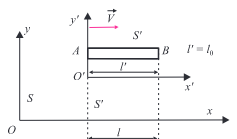
\includegraphics[width=0.5\textwidth]{fig/rigla} \\
    \figcaption{1.4}{Contractarea lungimilor. Rigla este solidară cu $S'$}
\end{figure}

\par
Din \( x' = \dfrac{x - Vt}{\lorentzradical} \)
rezultă \( x = x' \lorentzradical + Vt \). Atunci
\begin{align*}
    l &= x_2' \lorentzradical + Vt - x_1' \lorentzradical - Vt \\
    l &= (x_2' - x_1') \lorentzradical = l_0 \lorentzradical
\end{align*}

\vspace{1cm}

\par
Dimensiunile transversale ale corpurilor nu se modifică: \( y' = y \) și \( z' = z \).
Astfel, volumul corpului se modifică doar în direcția mișcării.
\[ \mathscr{V}_0 = xyz \]
\[ \mathscr{V}' = x'y'z' = x\lorentzradical yz = \mathscr{V}_0 \lorentzradical \]

\begin{wrapfigure}{r}{0.5\textwidth}
    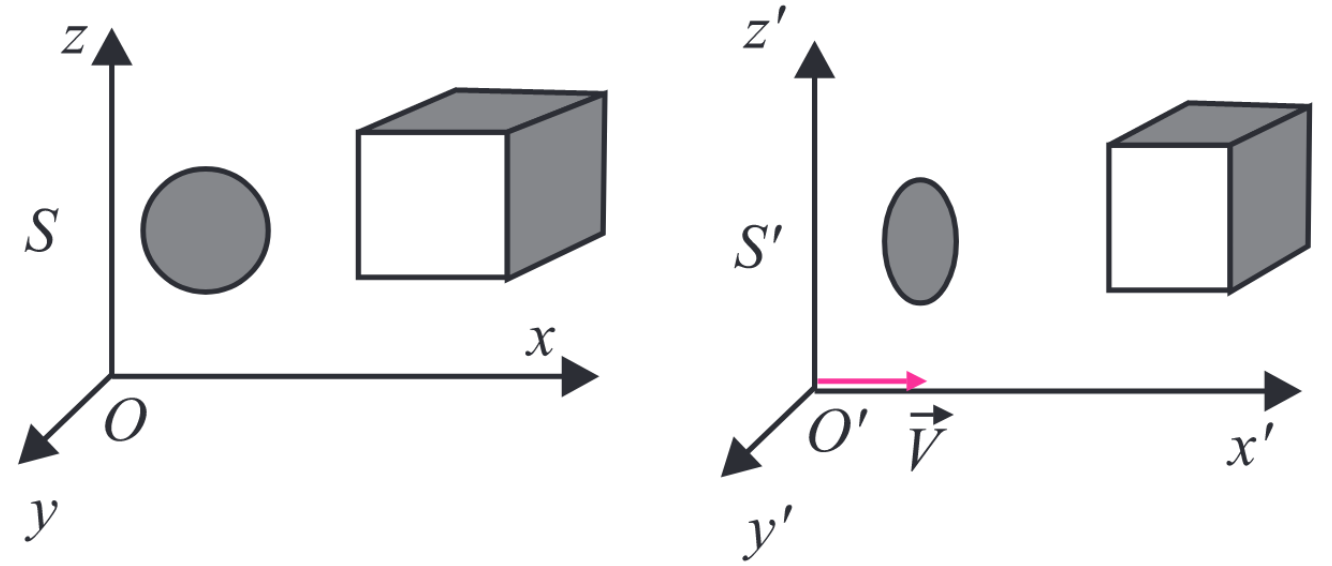
\includegraphics[width=0.5\textwidth]{fig/turtit.png}
    \figcaption{2}{Sfera se turtește, iar cubul devine paralelipiped}
\end{wrapfigure}

Privind o sferă dintr-un sistem de referință față de care se mișcă, aceasta
apare turtită în direcția mișcării. Un cub devine un paralelipiped.
Aceste modificări reprezintă forma reală a obiectelor, nu doar ceea ce vede
un observator. Imaginea adevărată a corpului poate fi obținută numai prin
localizarea simultană a tuturor punctelor acestuia. Atunci când observăm un
obiect în mișcare rapidă, în realitate înregistrăm fotonii emiși de obiect
atunci când ajung pe retină. Fotonii nu au fost emiși simultan de toate punctele
corpului, și astfel ochiul percepe o imagine deformată.

\end{document}
